\documentclass[1p]{elsarticle_modified}
%\bibliographystyle{elsarticle-num}

%\usepackage[colorlinks]{hyperref}
%\usepackage{abbrmath_seonhwa} %\Abb, \Ascr, \Acal ,\Abf, \Afrak
\usepackage{amsfonts}
\usepackage{amssymb}
\usepackage{amsmath}
\usepackage{amsthm}
\usepackage{scalefnt}
\usepackage{amsbsy}
\usepackage{kotex}
\usepackage{caption}
\usepackage{subfig}
\usepackage{color}
\usepackage{graphicx}
\usepackage{xcolor} %% white, black, red, green, blue, cyan, magenta, yellow
\usepackage{float}
\usepackage{setspace}
\usepackage{hyperref}

\usepackage{tikz}
\usetikzlibrary{arrows}

\usepackage{multirow}
\usepackage{array} % fixed length table
\usepackage{hhline}

%%%%%%%%%%%%%%%%%%%%%
\makeatletter
\renewcommand*\env@matrix[1][\arraystretch]{%
	\edef\arraystretch{#1}%
	\hskip -\arraycolsep
	\let\@ifnextchar\new@ifnextchar
	\array{*\c@MaxMatrixCols c}}
\makeatother %https://tex.stackexchange.com/questions/14071/how-can-i-increase-the-line-spacing-in-a-matrix
%%%%%%%%%%%%%%%

\usepackage[normalem]{ulem}

\newcommand{\msout}[1]{\ifmmode\text{\sout{\ensuremath{#1}}}\else\sout{#1}\fi}
%SOURCE: \msout is \stkout macro in https://tex.stackexchange.com/questions/20609/strikeout-in-math-mode

\newcommand{\cancel}[1]{
	\ifmmode
	{\color{red}\msout{#1}}
	\else
	{\color{red}\sout{#1}}
	\fi
}

\newcommand{\add}[1]{
	{\color{blue}\uwave{#1}}
}

\newcommand{\replace}[2]{
	\ifmmode
	{\color{red}\msout{#1}}{\color{blue}\uwave{#2}}
	\else
	{\color{red}\sout{#1}}{\color{blue}\uwave{#2}}
	\fi
}

\newcommand{\Sol}{\mathcal{S}} %segment
\newcommand{\D}{D} %diagram
\newcommand{\A}{\mathcal{A}} %arc


%%%%%%%%%%%%%%%%%%%%%%%%%%%%%5 test

\def\sl{\operatorname{\textup{SL}}(2,\Cbb)}
\def\psl{\operatorname{\textup{PSL}}(2,\Cbb)}
\def\quan{\mkern 1mu \triangleright \mkern 1mu}

\theoremstyle{definition}
\newtheorem{thm}{Theorem}[section]
\newtheorem{prop}[thm]{Proposition}
\newtheorem{lem}[thm]{Lemma}
\newtheorem{ques}[thm]{Question}
\newtheorem{cor}[thm]{Corollary}
\newtheorem{defn}[thm]{Definition}
\newtheorem{exam}[thm]{Example}
\newtheorem{rmk}[thm]{Remark}
\newtheorem{alg}[thm]{Algorithm}

\newcommand{\I}{\sqrt{-1}}
\begin{document}

%\begin{frontmatter}
%
%\title{Boundary parabolic representations of knots up to 8 crossings}
%
%%% Group authors per affiliation:
%\author{Yunhi Cho} 
%\address{Department of Mathematics, University of Seoul, Seoul, Korea}
%\ead{yhcho@uos.ac.kr}
%
%
%\author{Seonhwa Kim} %\fnref{s_kim}}
%\address{Center for Geometry and Physics, Institute for Basic Science, Pohang, 37673, Korea}
%\ead{ryeona17@ibs.re.kr}
%
%\author{Hyuk Kim}
%\address{Department of Mathematical Sciences, Seoul National University, Seoul 08826, Korea}
%\ead{hyukkim@snu.ac.kr}
%
%\author{Seokbeom Yoon}
%\address{Department of Mathematical Sciences, Seoul National University, Seoul, 08826,  Korea}
%\ead{sbyoon15@snu.ac.kr}
%
%\begin{abstract}
%We find all boundary parabolic representation of knots up to 8 crossings.
%
%\end{abstract}
%\begin{keyword}
%    \MSC[2010] 57M25 
%\end{keyword}
%
%\end{frontmatter}

%\linenumbers
%\tableofcontents
%
\newcommand\colored[1]{\textcolor{white}{\rule[-0.35ex]{0.8em}{1.4ex}}\kern-0.8em\color{red} #1}%
%\newcommand\colored[1]{\textcolor{white}{ #1}\kern-2.17ex	\textcolor{white}{ #1}\kern-1.81ex	\textcolor{white}{ #1}\kern-2.15ex\color{red}#1	}

{\Large $\underline{12n_{0609}~(K12n_{0609})}$}

\setlength{\tabcolsep}{10pt}
\renewcommand{\arraystretch}{1.6}
\vspace{1cm}\begin{tabular}{m{100pt}>{\centering\arraybackslash}m{274pt}}
\multirow{5}{120pt}{
	\centering
	\includegraphics[width=112pt]{../../../GIT/diagram.site/Diagrams/png/2698_12n_0609.png}\\
\ \ \ A knot diagram\footnotemark}&
\allowdisplaybreaks
\textbf{Linearized knot diagam} \\
\cline{2-2}
 &
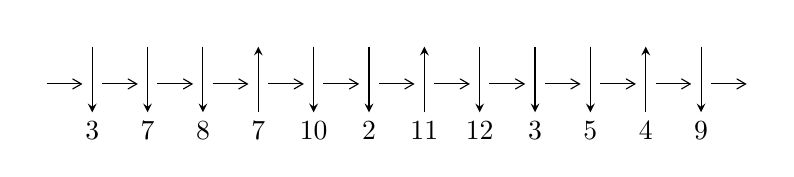
\begin{tikzpicture}[x=20pt, y=17pt]
	% nodes
	\node (C0) at (0, 0) {};
	\node (C1) at (1, 0) {};
	\node (C1U) at (1, +1) {};
	\node (C1D) at (1, -1) {3};

	\node (C2) at (2, 0) {};
	\node (C2U) at (2, +1) {};
	\node (C2D) at (2, -1) {7};

	\node (C3) at (3, 0) {};
	\node (C3U) at (3, +1) {};
	\node (C3D) at (3, -1) {8};

	\node (C4) at (4, 0) {};
	\node (C4U) at (4, +1) {};
	\node (C4D) at (4, -1) {7};

	\node (C5) at (5, 0) {};
	\node (C5U) at (5, +1) {};
	\node (C5D) at (5, -1) {10};

	\node (C6) at (6, 0) {};
	\node (C6U) at (6, +1) {};
	\node (C6D) at (6, -1) {2};

	\node (C7) at (7, 0) {};
	\node (C7U) at (7, +1) {};
	\node (C7D) at (7, -1) {11};

	\node (C8) at (8, 0) {};
	\node (C8U) at (8, +1) {};
	\node (C8D) at (8, -1) {12};

	\node (C9) at (9, 0) {};
	\node (C9U) at (9, +1) {};
	\node (C9D) at (9, -1) {3};

	\node (C10) at (10, 0) {};
	\node (C10U) at (10, +1) {};
	\node (C10D) at (10, -1) {5};

	\node (C11) at (11, 0) {};
	\node (C11U) at (11, +1) {};
	\node (C11D) at (11, -1) {4};

	\node (C12) at (12, 0) {};
	\node (C12U) at (12, +1) {};
	\node (C12D) at (12, -1) {9};
	\node (C13) at (13, 0) {};

	% arrows
	\draw[->,>={angle 60}]
	(C0) edge (C1) (C1) edge (C2) (C2) edge (C3) (C3) edge (C4) (C4) edge (C5) (C5) edge (C6) (C6) edge (C7) (C7) edge (C8) (C8) edge (C9) (C9) edge (C10) (C10) edge (C11) (C11) edge (C12) (C12) edge (C13) ;	\draw[->,>=stealth]
	(C1U) edge (C1D) (C2U) edge (C2D) (C3U) edge (C3D) (C4D) edge (C4U) (C5U) edge (C5D) (C6U) edge (C6D) (C7D) edge (C7U) (C8U) edge (C8D) (C9U) edge (C9D) (C10U) edge (C10D) (C11D) edge (C11U) (C12U) edge (C12D) ;
	\end{tikzpicture} \\
\hhline{~~} \\& 
\textbf{Solving Sequence} \\ \cline{2-2} 
 &
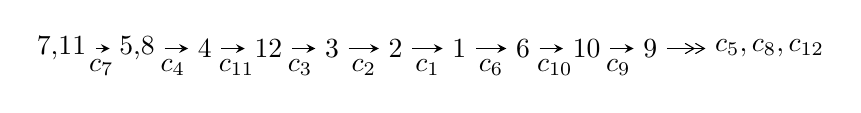
\begin{tikzpicture}[x=23pt, y=7pt]
	% node
	\node (A0) at (-1/8, 0) {7,11};
	\node (A1) at (17/16, 0) {5,8};
	\node (A2) at (17/8, 0) {4};
	\node (A3) at (25/8, 0) {12};
	\node (A4) at (33/8, 0) {3};
	\node (A5) at (41/8, 0) {2};
	\node (A6) at (49/8, 0) {1};
	\node (A7) at (57/8, 0) {6};
	\node (A8) at (65/8, 0) {10};
	\node (A9) at (73/8, 0) {9};
	\node (C1) at (1/2, -1) {$c_{7}$};
	\node (C2) at (13/8, -1) {$c_{4}$};
	\node (C3) at (21/8, -1) {$c_{11}$};
	\node (C4) at (29/8, -1) {$c_{3}$};
	\node (C5) at (37/8, -1) {$c_{2}$};
	\node (C6) at (45/8, -1) {$c_{1}$};
	\node (C7) at (53/8, -1) {$c_{6}$};
	\node (C8) at (61/8, -1) {$c_{10}$};
	\node (C9) at (69/8, -1) {$c_{9}$};
	\node (A10) at (11, 0) {$c_{5},c_{8},c_{12}$};

	% edge
	\draw[->,>=stealth]	
	(A0) edge (A1) (A1) edge (A2) (A2) edge (A3) (A3) edge (A4) (A4) edge (A5) (A5) edge (A6) (A6) edge (A7) (A7) edge (A8) (A8) edge (A9) ;
	\draw[->>,>={angle 60}]	
	(A9) edge (A10);
\end{tikzpicture} \\ 

\end{tabular} \\

\footnotetext{
The image of knot diagram is generated by the software ``\textbf{Draw programme}" developed by Andrew Bartholomew(\url{http://www.layer8.co.uk/maths/draw/index.htm\#Running-draw}), where we modified some parts for our purpose(\url{https://github.com/CATsTAILs/LinksPainter}).
}\phantom \\ \newline 
\centering \textbf{Ideals for irreducible components\footnotemark of $X_{\text{par}}$} 
 
\begin{align*}
I^u_{1}&=\langle 
4.50523\times10^{31} u^{34}+3.77516\times10^{31} u^{33}+\cdots+2.98297\times10^{32} b+5.56578\times10^{32},\\
\phantom{I^u_{1}}&\phantom{= \langle  }1.58581\times10^{33} u^{34}-2.10588\times10^{32} u^{33}+\cdots+2.08808\times10^{33} a-7.24786\times10^{33},\;u^{35}-7 u^{33}+\cdots-15 u-7\rangle \\
I^u_{2}&=\langle 
-3 u^{13}+4 u^{12}+12 u^{11}-14 u^{10}-24 u^9+33 u^8+22 u^7-41 u^6-4 u^5+33 u^4-8 u^3-16 u^2+b+5 u+5,\\
\phantom{I^u_{2}}&\phantom{= \langle  }u^{13}- u^{12}-4 u^{11}+3 u^{10}+8 u^9-8 u^8-8 u^7+10 u^6+3 u^5-10 u^4+u^3+4 u^2+a- u-2,\\
\phantom{I^u_{2}}&\phantom{= \langle  }u^{15}- u^{14}-5 u^{13}+4 u^{12}+12 u^{11}-11 u^{10}-16 u^9+18 u^8+11 u^7-20 u^6-2 u^5+14 u^4-2 u^3-6 u^2+u+1\rangle \\
\\
\end{align*}
\raggedright * 2 irreducible components of $\dim_{\mathbb{C}}=0$, with total 50 representations.\\
\footnotetext{All coefficients of polynomials are rational numbers. But the coefficients are sometimes approximated in decimal forms when there is not enough margin.}
\newpage
\renewcommand{\arraystretch}{1}
\centering \section*{I. $I^u_{1}= \langle 4.51\times10^{31} u^{34}+3.78\times10^{31} u^{33}+\cdots+2.98\times10^{32} b+5.57\times10^{32},\;1.59\times10^{33} u^{34}-2.11\times10^{32} u^{33}+\cdots+2.09\times10^{33} a-7.25\times10^{33},\;u^{35}-7 u^{33}+\cdots-15 u-7 \rangle$}
\flushleft \textbf{(i) Arc colorings}\\
\begin{tabular}{m{7pt} m{180pt} m{7pt} m{180pt} }
\flushright $a_{7}=$&$\begin{pmatrix}1\\0\end{pmatrix}$ \\
\flushright $a_{11}=$&$\begin{pmatrix}0\\u\end{pmatrix}$ \\
\flushright $a_{5}=$&$\begin{pmatrix}-0.759458 u^{34}+0.100853 u^{33}+\cdots-4.69237 u+3.47107\\-0.151032 u^{34}-0.126557 u^{33}+\cdots-11.7344 u-1.86585\end{pmatrix}$ \\
\flushright $a_{8}=$&$\begin{pmatrix}1\\- u^2\end{pmatrix}$ \\
\flushright $a_{4}=$&$\begin{pmatrix}-0.608426 u^{34}+0.227410 u^{33}+\cdots+7.04204 u+5.33692\\-0.151032 u^{34}-0.126557 u^{33}+\cdots-11.7344 u-1.86585\end{pmatrix}$ \\
\flushright $a_{12}=$&$\begin{pmatrix}0.179494 u^{34}-0.738948 u^{33}+\cdots-15.5941 u-1.11702\\-0.545677 u^{34}+0.0968206 u^{33}+\cdots-9.38307 u+0.549020\end{pmatrix}$ \\
\flushright $a_{3}=$&$\begin{pmatrix}-1.02030 u^{34}+0.148917 u^{33}+\cdots-5.54020 u+5.06294\\-0.0217840 u^{34}-0.0983476 u^{33}+\cdots-7.67390 u-1.31640\end{pmatrix}$ \\
\flushright $a_{2}=$&$\begin{pmatrix}-1.04208 u^{34}+0.0505690 u^{33}+\cdots-13.2141 u+3.74654\\-0.0217840 u^{34}-0.0983476 u^{33}+\cdots-7.67390 u-1.31640\end{pmatrix}$ \\
\flushright $a_{1}=$&$\begin{pmatrix}0.840961 u^{34}-1.49063 u^{33}+\cdots-33.0344 u-11.5939\\-0.517267 u^{34}+0.810261 u^{33}+\cdots+18.9933 u+12.5715\end{pmatrix}$ \\
\flushright $a_{6}=$&$\begin{pmatrix}-0.851085 u^{34}-0.116346 u^{33}+\cdots-25.8199 u-1.77087\\0.0725660 u^{34}-0.436813 u^{33}+\cdots-17.0168 u-7.55024\end{pmatrix}$ \\
\flushright $a_{10}=$&$\begin{pmatrix}-0.456623 u^{34}-0.375284 u^{33}+\cdots-20.0850 u+2.76419\\-0.0904401 u^{34}+0.266844 u^{33}+\cdots+6.89220 u+3.33219\end{pmatrix}$ \\
\flushright $a_{9}=$&$\begin{pmatrix}-3.40594 u^{34}+1.42898 u^{33}+\cdots-12.4503 u+24.3578\\1.40463 u^{34}-0.957154 u^{33}+\cdots-5.03678 u-8.25778\end{pmatrix}$\\&\end{tabular}
\flushleft \textbf{(ii) Obstruction class $= -1$}\\~\\
\flushleft \textbf{(iii) Cusp Shapes $= 1.81804 u^{34}+1.88122 u^{33}+\cdots+110.974 u+25.9634$}\\~\\
\newpage\renewcommand{\arraystretch}{1}
\flushleft \textbf{(iv) u-Polynomials at the component}\newline \\
\begin{tabular}{m{50pt}|m{274pt}}
Crossings & \hspace{64pt}u-Polynomials at each crossing \\
\hline $$\begin{aligned}c_{1}\end{aligned}$$&$\begin{aligned}
&u^{35}+62 u^{34}+\cdots+4330075 u+134689
\end{aligned}$\\
\hline $$\begin{aligned}c_{2},c_{6}\end{aligned}$$&$\begin{aligned}
&u^{35}+2 u^{34}+\cdots+4061 u-367
\end{aligned}$\\
\hline $$\begin{aligned}c_{3}\end{aligned}$$&$\begin{aligned}
&u^{35}+2 u^{34}+\cdots-7 u+1
\end{aligned}$\\
\hline $$\begin{aligned}c_{4}\end{aligned}$$&$\begin{aligned}
&u^{35}+10 u^{34}+\cdots+1712 u+311
\end{aligned}$\\
\hline $$\begin{aligned}c_{5},c_{10}\end{aligned}$$&$\begin{aligned}
&u^{35}- u^{34}+\cdots+672 u-23
\end{aligned}$\\
\hline $$\begin{aligned}c_{7}\end{aligned}$$&$\begin{aligned}
&u^{35}-7 u^{33}+\cdots-15 u+7
\end{aligned}$\\
\hline $$\begin{aligned}c_{8},c_{12}\end{aligned}$$&$\begin{aligned}
&u^{35}+3 u^{34}+\cdots-97 u+19
\end{aligned}$\\
\hline $$\begin{aligned}c_{9}\end{aligned}$$&$\begin{aligned}
&u^{35}+4 u^{34}+\cdots-54708 u+6023
\end{aligned}$\\
\hline $$\begin{aligned}c_{11}\end{aligned}$$&$\begin{aligned}
&u^{35}-5 u^{34}+\cdots+422 u-13
\end{aligned}$\\
\hline
\end{tabular}\\~\\
\newpage\renewcommand{\arraystretch}{1}
\flushleft \textbf{(v) Riley Polynomials at the component}\newline \\
\begin{tabular}{m{50pt}|m{274pt}}
Crossings & \hspace{64pt}Riley Polynomials at each crossing \\
\hline $$\begin{aligned}c_{1}\end{aligned}$$&$\begin{aligned}
&y^{35}-206 y^{34}+\cdots+2682621801371 y-18141126721
\end{aligned}$\\
\hline $$\begin{aligned}c_{2},c_{6}\end{aligned}$$&$\begin{aligned}
&y^{35}-62 y^{34}+\cdots+4330075 y-134689
\end{aligned}$\\
\hline $$\begin{aligned}c_{3}\end{aligned}$$&$\begin{aligned}
&y^{35}+2 y^{34}+\cdots+63 y-1
\end{aligned}$\\
\hline $$\begin{aligned}c_{4}\end{aligned}$$&$\begin{aligned}
&y^{35}+10 y^{34}+\cdots-500008 y-96721
\end{aligned}$\\
\hline $$\begin{aligned}c_{5},c_{10}\end{aligned}$$&$\begin{aligned}
&y^{35}-3 y^{34}+\cdots+454344 y-529
\end{aligned}$\\
\hline $$\begin{aligned}c_{7}\end{aligned}$$&$\begin{aligned}
&y^{35}-14 y^{34}+\cdots+1023 y-49
\end{aligned}$\\
\hline $$\begin{aligned}c_{8},c_{12}\end{aligned}$$&$\begin{aligned}
&y^{35}-55 y^{34}+\cdots+11689 y-361
\end{aligned}$\\
\hline $$\begin{aligned}c_{9}\end{aligned}$$&$\begin{aligned}
&y^{35}-164 y^{34}+\cdots-17527853484 y-36276529
\end{aligned}$\\
\hline $$\begin{aligned}c_{11}\end{aligned}$$&$\begin{aligned}
&y^{35}+9 y^{34}+\cdots+217500 y-169
\end{aligned}$\\
\hline
\end{tabular}\\~\\
\newpage\flushleft \textbf{(vi) Complex Volumes and Cusp Shapes}
$$\begin{array}{c|c|c}  
\text{Solutions to }I^u_{1}& \I (\text{vol} + \sqrt{-1}CS) & \text{Cusp shape}\\
 \hline 
\begin{aligned}
u &= -0.675365 + 0.752140 I \\
a &= \phantom{-}0.274011 + 1.179370 I \\
b &= -0.55916 + 1.59846 I\end{aligned}
 & -5.38269 - 0.91248 I & -10.44886 + 2.53258 I \\ \hline\begin{aligned}
u &= -0.675365 - 0.752140 I \\
a &= \phantom{-}0.274011 - 1.179370 I \\
b &= -0.55916 - 1.59846 I\end{aligned}
 & -5.38269 + 0.91248 I & -10.44886 - 2.53258 I \\ \hline\begin{aligned}
u &= -0.928230\phantom{ +0.000000I} \\
a &= -0.743205\phantom{ +0.000000I} \\
b &= -3.28718\phantom{ +0.000000I}\end{aligned}
 & -10.2373\phantom{ +0.000000I} & -6.48310\phantom{ +0.000000I} \\ \hline\begin{aligned}
u &= -0.780540 + 0.794419 I \\
a &= \phantom{-}0.528114 + 0.428245 I \\
b &= -0.454633 + 0.505577 I\end{aligned}
 & -0.06975 - 2.50434 I & -7.09658 + 4.10230 I \\ \hline\begin{aligned}
u &= -0.780540 - 0.794419 I \\
a &= \phantom{-}0.528114 - 0.428245 I \\
b &= -0.454633 - 0.505577 I\end{aligned}
 & -0.06975 + 2.50434 I & -7.09658 - 4.10230 I \\ \hline\begin{aligned}
u &= -1.170970 + 0.199419 I \\
a &= \phantom{-}0.109806 - 0.892494 I \\
b &= \phantom{-}0.256411 - 0.529286 I\end{aligned}
 & \phantom{-}2.93670 - 2.65045 I & -2.92426 + 3.85701 I \\ \hline\begin{aligned}
u &= -1.170970 - 0.199419 I \\
a &= \phantom{-}0.109806 + 0.892494 I \\
b &= \phantom{-}0.256411 + 0.529286 I\end{aligned}
 & \phantom{-}2.93670 + 2.65045 I & -2.92426 - 3.85701 I \\ \hline\begin{aligned}
u &= -1.027690 + 0.614606 I \\
a &= -0.911917 - 0.413858 I \\
b &= \phantom{-}0.40767 - 1.44351 I\end{aligned}
 & -4.22355 - 4.34323 I & -8.88159 + 4.48072 I \\ \hline\begin{aligned}
u &= -1.027690 - 0.614606 I \\
a &= -0.911917 + 0.413858 I \\
b &= \phantom{-}0.40767 + 1.44351 I\end{aligned}
 & -4.22355 + 4.34323 I & -8.88159 - 4.48072 I \\ \hline\begin{aligned}
u &= -0.790308\phantom{ +0.000000I} \\
a &= \phantom{-}1.93557\phantom{ +0.000000I} \\
b &= -2.52371\phantom{ +0.000000I}\end{aligned}
 & -10.8736\phantom{ +0.000000I} & \phantom{-}0.541730\phantom{ +0.000000I}\\
 \hline 
 \end{array}$$\newpage$$\begin{array}{c|c|c}  
\text{Solutions to }I^u_{1}& \I (\text{vol} + \sqrt{-1}CS) & \text{Cusp shape}\\
 \hline 
\begin{aligned}
u &= \phantom{-}0.779444 + 0.122722 I \\
a &= \phantom{-}0.11921 + 1.82402 I \\
b &= \phantom{-}0.692344 + 0.750731 I\end{aligned}
 & \phantom{-}4.75580 + 0.44115 I & -1.38131 + 2.20530 I \\ \hline\begin{aligned}
u &= \phantom{-}0.779444 - 0.122722 I \\
a &= \phantom{-}0.11921 - 1.82402 I \\
b &= \phantom{-}0.692344 - 0.750731 I\end{aligned}
 & \phantom{-}4.75580 - 0.44115 I & -1.38131 - 2.20530 I \\ \hline\begin{aligned}
u &= \phantom{-}1.097490 + 0.543646 I \\
a &= -0.208642 + 0.776842 I \\
b &= \phantom{-}0.97202 + 1.45913 I\end{aligned}
 & \phantom{-}1.07838 + 5.16629 I & -6.84650 - 9.62882 I \\ \hline\begin{aligned}
u &= \phantom{-}1.097490 - 0.543646 I \\
a &= -0.208642 - 0.776842 I \\
b &= \phantom{-}0.97202 - 1.45913 I\end{aligned}
 & \phantom{-}1.07838 - 5.16629 I & -6.84650 + 9.62882 I \\ \hline\begin{aligned}
u &= \phantom{-}0.879026 + 0.883079 I \\
a &= -1.65073 + 0.15661 I \\
b &= -0.276490 + 0.900117 I\end{aligned}
 & -16.3550 + 2.1833 I & -9.12494 - 2.49613 I \\ \hline\begin{aligned}
u &= \phantom{-}0.879026 - 0.883079 I \\
a &= -1.65073 - 0.15661 I \\
b &= -0.276490 - 0.900117 I\end{aligned}
 & -16.3550 - 2.1833 I & -9.12494 + 2.49613 I \\ \hline\begin{aligned}
u &= -1.004900 + 0.750402 I \\
a &= \phantom{-}0.159109 - 0.878002 I \\
b &= \phantom{-}0.886553 - 0.937980 I\end{aligned}
 & \phantom{-}0.76221 - 3.35277 I & -9.00923 + 1.04834 I \\ \hline\begin{aligned}
u &= -1.004900 - 0.750402 I \\
a &= \phantom{-}0.159109 + 0.878002 I \\
b &= \phantom{-}0.886553 + 0.937980 I\end{aligned}
 & \phantom{-}0.76221 + 3.35277 I & -9.00923 - 1.04834 I \\ \hline\begin{aligned}
u &= \phantom{-}0.980302 + 0.839353 I \\
a &= -0.12512 - 1.44580 I \\
b &= -0.56077 - 1.91870 I\end{aligned}
 & -16.0274 + 4.2362 I & -8.99278 - 2.47237 I \\ \hline\begin{aligned}
u &= \phantom{-}0.980302 - 0.839353 I \\
a &= -0.12512 + 1.44580 I \\
b &= -0.56077 + 1.91870 I\end{aligned}
 & -16.0274 - 4.2362 I & -8.99278 + 2.47237 I\\
 \hline 
 \end{array}$$\newpage$$\begin{array}{c|c|c}  
\text{Solutions to }I^u_{1}& \I (\text{vol} + \sqrt{-1}CS) & \text{Cusp shape}\\
 \hline 
\begin{aligned}
u &= \phantom{-}0.371475 + 0.598922 I \\
a &= \phantom{-}0.882706 - 0.414519 I \\
b &= -0.207818 - 0.631352 I\end{aligned}
 & -1.039020 - 0.567157 I & -9.02941 + 3.66448 I \\ \hline\begin{aligned}
u &= \phantom{-}0.371475 - 0.598922 I \\
a &= \phantom{-}0.882706 + 0.414519 I \\
b &= -0.207818 + 0.631352 I\end{aligned}
 & -1.039020 + 0.567157 I & -9.02941 - 3.66448 I \\ \hline\begin{aligned}
u &= \phantom{-}0.663303\phantom{ +0.000000I} \\
a &= \phantom{-}1.17343\phantom{ +0.000000I} \\
b &= -0.625094\phantom{ +0.000000I}\end{aligned}
 & -1.52399\phantom{ +0.000000I} & -5.20750\phantom{ +0.000000I} \\ \hline\begin{aligned}
u &= \phantom{-}1.019370 + 0.891636 I \\
a &= \phantom{-}0.374425 - 0.936128 I \\
b &= -0.81320 - 1.16561 I\end{aligned}
 & -4.62293 + 8.02466 I & -8.99459 - 6.09889 I \\ \hline\begin{aligned}
u &= \phantom{-}1.019370 - 0.891636 I \\
a &= \phantom{-}0.374425 + 0.936128 I \\
b &= -0.81320 + 1.16561 I\end{aligned}
 & -4.62293 - 8.02466 I & -8.99459 + 6.09889 I \\ \hline\begin{aligned}
u &= -0.625529 + 1.237630 I \\
a &= -1.149750 - 0.604247 I \\
b &= -0.498371 - 1.184570 I\end{aligned}
 & -17.6881 + 5.3333 I & -10.32662 - 2.48689 I \\ \hline\begin{aligned}
u &= -0.625529 - 1.237630 I \\
a &= -1.149750 + 0.604247 I \\
b &= -0.498371 + 1.184570 I\end{aligned}
 & -17.6881 - 5.3333 I & -10.32662 + 2.48689 I \\ \hline\begin{aligned}
u &= \phantom{-}0.936546 + 1.042190 I \\
a &= -0.390412 + 0.550295 I \\
b &= -0.114051 + 0.985066 I\end{aligned}
 & -5.01490 - 1.02895 I & -12.04957 + 2.53411 I \\ \hline\begin{aligned}
u &= \phantom{-}0.936546 - 1.042190 I \\
a &= -0.390412 - 0.550295 I \\
b &= -0.114051 - 0.985066 I\end{aligned}
 & -5.01490 + 1.02895 I & -12.04957 - 2.53411 I \\ \hline\begin{aligned}
u &= \phantom{-}0.587494\phantom{ +0.000000I} \\
a &= -0.0584535\phantom{ +0.000000I} \\
b &= -1.70895\phantom{ +0.000000I}\end{aligned}
 & -2.29968\phantom{ +0.000000I} & \phantom{-}3.86260\phantom{ +0.000000I}\\
 \hline 
 \end{array}$$\newpage$$\begin{array}{c|c|c}  
\text{Solutions to }I^u_{1}& \I (\text{vol} + \sqrt{-1}CS) & \text{Cusp shape}\\
 \hline 
\begin{aligned}
u &= -1.22874 + 0.83593 I \\
a &= \phantom{-}0.186277 + 1.290050 I \\
b &= -1.04714 + 1.80529 I\end{aligned}
 & -15.6932 - 12.6803 I & -6.00000 + 5.76735 I \\ \hline\begin{aligned}
u &= -1.22874 - 0.83593 I \\
a &= \phantom{-}0.186277 - 1.290050 I \\
b &= -1.04714 - 1.80529 I\end{aligned}
 & -15.6932 + 12.6803 I & -6.00000 - 5.76735 I \\ \hline\begin{aligned}
u &= -0.364021 + 0.159376 I \\
a &= -2.08592 + 2.84763 I \\
b &= \phantom{-}0.575909 + 0.656185 I\end{aligned}
 & -0.87711 - 2.42741 I & -7.50647 + 0.56307 I \\ \hline\begin{aligned}
u &= -0.364021 - 0.159376 I \\
a &= -2.08592 - 2.84763 I \\
b &= \phantom{-}0.575909 - 0.656185 I\end{aligned}
 & -0.87711 + 2.42741 I & -7.50647 - 0.56307 I \\ \hline\begin{aligned}
u &= \phantom{-}2.09595\phantom{ +0.000000I} \\
a &= -0.386813\phantom{ +0.000000I} \\
b &= -0.373598\phantom{ +0.000000I}\end{aligned}
 & -7.66684\phantom{ +0.000000I} & \phantom{-0.000000 } 0\\
 \hline 
 \end{array}$$\newpage\newpage\renewcommand{\arraystretch}{1}
\centering \section*{II. $I^u_{2}= \langle -3 u^{13}+4 u^{12}+\cdots+b+5,\;u^{13}- u^{12}+\cdots+a-2,\;u^{15}- u^{14}+\cdots+u+1 \rangle$}
\flushleft \textbf{(i) Arc colorings}\\
\begin{tabular}{m{7pt} m{180pt} m{7pt} m{180pt} }
\flushright $a_{7}=$&$\begin{pmatrix}1\\0\end{pmatrix}$ \\
\flushright $a_{11}=$&$\begin{pmatrix}0\\u\end{pmatrix}$ \\
\flushright $a_{5}=$&$\begin{pmatrix}- u^{13}+u^{12}+\cdots+u+2\\3 u^{13}-4 u^{12}+\cdots-5 u-5\end{pmatrix}$ \\
\flushright $a_{8}=$&$\begin{pmatrix}1\\- u^2\end{pmatrix}$ \\
\flushright $a_{4}=$&$\begin{pmatrix}-4 u^{13}+5 u^{12}+\cdots+6 u+7\\3 u^{13}-4 u^{12}+\cdots-5 u-5\end{pmatrix}$ \\
\flushright $a_{12}=$&$\begin{pmatrix}-15 u^{14}+12 u^{13}+\cdots+38 u+6\\7 u^{14}-4 u^{13}+\cdots-22 u-6\end{pmatrix}$ \\
\flushright $a_{3}=$&$\begin{pmatrix}u^{14}-5 u^{13}+\cdots+5 u+6\\3 u^{13}-3 u^{12}+\cdots-4 u-5\end{pmatrix}$ \\
\flushright $a_{2}=$&$\begin{pmatrix}u^{14}-2 u^{13}+\cdots+u+1\\3 u^{13}-3 u^{12}+\cdots-4 u-5\end{pmatrix}$ \\
\flushright $a_{1}=$&$\begin{pmatrix}20 u^{14}-13 u^{13}+\cdots-53 u-20\\-10 u^{14}+4 u^{13}+\cdots+32 u+12\end{pmatrix}$ \\
\flushright $a_{6}=$&$\begin{pmatrix}- u^{14}-3 u^{13}+\cdots+9 u+9\\4 u^{14}-3 u^{13}+\cdots-11 u-7\end{pmatrix}$ \\
\flushright $a_{10}=$&$\begin{pmatrix}-4 u^{14}+4 u^{13}+\cdots+5 u^2+6 u\\4 u^{14}-4 u^{13}+\cdots-9 u^2-8 u\end{pmatrix}$ \\
\flushright $a_{9}=$&$\begin{pmatrix}9 u^{14}+7 u^{13}+\cdots-53 u-30\\-7 u^{14}+37 u^{12}+\cdots+30 u+17\end{pmatrix}$\\&\end{tabular}
\flushleft \textbf{(ii) Obstruction class $= 1$}\\~\\
\flushleft \textbf{(iii) Cusp Shapes $= -4 u^{14}+19 u^{13}+5 u^{12}-83 u^{11}+6 u^{10}+184 u^9-78 u^8-223 u^7+161 u^6+135 u^5-187 u^4-27 u^3+108 u^2-9 u-37$}\\~\\
\newpage\renewcommand{\arraystretch}{1}
\flushleft \textbf{(iv) u-Polynomials at the component}\newline \\
\begin{tabular}{m{50pt}|m{274pt}}
Crossings & \hspace{64pt}u-Polynomials at each crossing \\
\hline $$\begin{aligned}c_{1}\end{aligned}$$&$\begin{aligned}
&u^{15}-15 u^{14}+\cdots+5 u-1
\end{aligned}$\\
\hline $$\begin{aligned}c_{2}\end{aligned}$$&$\begin{aligned}
&u^{15}-3 u^{14}+\cdots+3 u-1
\end{aligned}$\\
\hline $$\begin{aligned}c_{3}\end{aligned}$$&$\begin{aligned}
&u^{15}+u^{14}+\cdots+3 u+1
\end{aligned}$\\
\hline $$\begin{aligned}c_{4}\end{aligned}$$&$\begin{aligned}
&u^{15}+u^{14}+\cdots+2 u-1
\end{aligned}$\\
\hline $$\begin{aligned}c_{5}\end{aligned}$$&$\begin{aligned}
&u^{15}+6 u^{13}+\cdots-2 u-1
\end{aligned}$\\
\hline $$\begin{aligned}c_{6}\end{aligned}$$&$\begin{aligned}
&u^{15}+3 u^{14}+\cdots+3 u+1
\end{aligned}$\\
\hline $$\begin{aligned}c_{7}\end{aligned}$$&$\begin{aligned}
&u^{15}- u^{14}+\cdots+u+1
\end{aligned}$\\
\hline $$\begin{aligned}c_{8}\end{aligned}$$&$\begin{aligned}
&u^{15}-10 u^{13}+\cdots+u+1
\end{aligned}$\\
\hline $$\begin{aligned}c_{9}\end{aligned}$$&$\begin{aligned}
&u^{15}-5 u^{14}+\cdots-14 u+1
\end{aligned}$\\
\hline $$\begin{aligned}c_{10}\end{aligned}$$&$\begin{aligned}
&u^{15}+6 u^{13}+\cdots-2 u+1
\end{aligned}$\\
\hline $$\begin{aligned}c_{11}\end{aligned}$$&$\begin{aligned}
&u^{15}-2 u^{13}+\cdots-11 u^2-1
\end{aligned}$\\
\hline $$\begin{aligned}c_{12}\end{aligned}$$&$\begin{aligned}
&u^{15}-10 u^{13}+\cdots+u-1
\end{aligned}$\\
\hline
\end{tabular}\\~\\
\newpage\renewcommand{\arraystretch}{1}
\flushleft \textbf{(v) Riley Polynomials at the component}\newline \\
\begin{tabular}{m{50pt}|m{274pt}}
Crossings & \hspace{64pt}Riley Polynomials at each crossing \\
\hline $$\begin{aligned}c_{1}\end{aligned}$$&$\begin{aligned}
&y^{15}-59 y^{14}+\cdots+5 y-1
\end{aligned}$\\
\hline $$\begin{aligned}c_{2},c_{6}\end{aligned}$$&$\begin{aligned}
&y^{15}-15 y^{14}+\cdots+5 y-1
\end{aligned}$\\
\hline $$\begin{aligned}c_{3}\end{aligned}$$&$\begin{aligned}
&y^{15}+5 y^{14}+\cdots+17 y-1
\end{aligned}$\\
\hline $$\begin{aligned}c_{4}\end{aligned}$$&$\begin{aligned}
&y^{15}-7 y^{14}+\cdots-14 y-1
\end{aligned}$\\
\hline $$\begin{aligned}c_{5},c_{10}\end{aligned}$$&$\begin{aligned}
&y^{15}+12 y^{14}+\cdots-6 y-1
\end{aligned}$\\
\hline $$\begin{aligned}c_{7}\end{aligned}$$&$\begin{aligned}
&y^{15}-11 y^{14}+\cdots+13 y-1
\end{aligned}$\\
\hline $$\begin{aligned}c_{8},c_{12}\end{aligned}$$&$\begin{aligned}
&y^{15}-20 y^{14}+\cdots-9 y-1
\end{aligned}$\\
\hline $$\begin{aligned}c_{9}\end{aligned}$$&$\begin{aligned}
&y^{15}-53 y^{14}+\cdots+38 y-1
\end{aligned}$\\
\hline $$\begin{aligned}c_{11}\end{aligned}$$&$\begin{aligned}
&y^{15}-4 y^{14}+\cdots-22 y-1
\end{aligned}$\\
\hline
\end{tabular}\\~\\
\newpage\flushleft \textbf{(vi) Complex Volumes and Cusp Shapes}
$$\begin{array}{c|c|c}  
\text{Solutions to }I^u_{2}& \I (\text{vol} + \sqrt{-1}CS) & \text{Cusp shape}\\
 \hline 
\begin{aligned}
u &= -0.945967 + 0.364350 I \\
a &= \phantom{-}0.447371 - 1.296300 I \\
b &= \phantom{-}0.54568 - 1.59008 I\end{aligned}
 & \phantom{-}0.121261 + 0.585920 I & -6.11150 + 0.88466 I \\ \hline\begin{aligned}
u &= -0.945967 - 0.364350 I \\
a &= \phantom{-}0.447371 + 1.296300 I \\
b &= \phantom{-}0.54568 + 1.59008 I\end{aligned}
 & \phantom{-}0.121261 - 0.585920 I & -6.11150 - 0.88466 I \\ \hline\begin{aligned}
u &= \phantom{-}0.910844 + 0.329867 I \\
a &= \phantom{-}0.63588 + 1.36871 I \\
b &= \phantom{-}0.434324 + 0.641040 I\end{aligned}
 & \phantom{-}4.62454 + 1.37648 I & -3.28500 - 4.85991 I \\ \hline\begin{aligned}
u &= \phantom{-}0.910844 - 0.329867 I \\
a &= \phantom{-}0.63588 - 1.36871 I \\
b &= \phantom{-}0.434324 - 0.641040 I\end{aligned}
 & \phantom{-}4.62454 - 1.37648 I & -3.28500 + 4.85991 I \\ \hline\begin{aligned}
u &= \phantom{-}0.483149 + 0.790685 I \\
a &= \phantom{-}0.552124 + 0.303102 I \\
b &= -0.006540 - 0.521541 I\end{aligned}
 & -3.32772 - 1.16564 I & -9.43576 + 1.29116 I \\ \hline\begin{aligned}
u &= \phantom{-}0.483149 - 0.790685 I \\
a &= \phantom{-}0.552124 - 0.303102 I \\
b &= -0.006540 + 0.521541 I\end{aligned}
 & -3.32772 + 1.16564 I & -9.43576 - 1.29116 I \\ \hline\begin{aligned}
u &= -0.858047 + 0.316539 I \\
a &= \phantom{-}0.85127 - 1.27055 I \\
b &= -0.183732 + 0.291743 I\end{aligned}
 & -0.26649 - 3.45017 I & -3.88329 + 5.28365 I \\ \hline\begin{aligned}
u &= -0.858047 - 0.316539 I \\
a &= \phantom{-}0.85127 + 1.27055 I \\
b &= -0.183732 - 0.291743 I\end{aligned}
 & -0.26649 + 3.45017 I & -3.88329 - 5.28365 I \\ \hline\begin{aligned}
u &= \phantom{-}1.047160 + 0.587752 I \\
a &= \phantom{-}0.157821 + 0.780474 I \\
b &= \phantom{-}1.54439 + 1.24046 I\end{aligned}
 & -1.69704 + 6.28081 I & -7.36459 - 5.95096 I \\ \hline\begin{aligned}
u &= \phantom{-}1.047160 - 0.587752 I \\
a &= \phantom{-}0.157821 - 0.780474 I \\
b &= \phantom{-}1.54439 - 1.24046 I\end{aligned}
 & -1.69704 - 6.28081 I & -7.36459 + 5.95096 I\\
 \hline 
 \end{array}$$\newpage$$\begin{array}{c|c|c}  
\text{Solutions to }I^u_{2}& \I (\text{vol} + \sqrt{-1}CS) & \text{Cusp shape}\\
 \hline 
\begin{aligned}
u &= \phantom{-}0.686348\phantom{ +0.000000I} \\
a &= \phantom{-}1.89062\phantom{ +0.000000I} \\
b &= -3.01568\phantom{ +0.000000I}\end{aligned}
 & -11.2981\phantom{ +0.000000I} & -19.7640\phantom{ +0.000000I} \\ \hline\begin{aligned}
u &= -1.189670 + 0.653681 I \\
a &= \phantom{-}0.004952 - 0.642912 I \\
b &= \phantom{-}0.747056 - 0.985367 I\end{aligned}
 & \phantom{-}1.40673 - 4.12593 I & -4.27551 + 5.62522 I \\ \hline\begin{aligned}
u &= -1.189670 - 0.653681 I \\
a &= \phantom{-}0.004952 + 0.642912 I \\
b &= \phantom{-}0.747056 + 0.985367 I\end{aligned}
 & \phantom{-}1.40673 + 4.12593 I & -4.27551 - 5.62522 I \\ \hline\begin{aligned}
u &= -0.428593\phantom{ +0.000000I} \\
a &= \phantom{-}1.22503\phantom{ +0.000000I} \\
b &= -1.45207\phantom{ +0.000000I}\end{aligned}
 & -2.69518\phantom{ +0.000000I} & -18.0200\phantom{ +0.000000I} \\ \hline\begin{aligned}
u &= \phantom{-}1.84731\phantom{ +0.000000I} \\
a &= -0.414496\phantom{ +0.000000I} \\
b &= -0.694610\phantom{ +0.000000I}\end{aligned}
 & -7.46852\phantom{ +0.000000I} & \phantom{-}5.49540\phantom{ +0.000000I}\\
 \hline 
 \end{array}$$\newpage
\newpage\renewcommand{\arraystretch}{1}
\centering \section*{ III. u-Polynomials}
\begin{tabular}{m{50pt}|m{274pt}}
Crossings & \hspace{64pt}u-Polynomials at each crossing \\
\hline $$\begin{aligned}c_{1}\end{aligned}$$&$\begin{aligned}
&(u^{15}-15 u^{14}+\cdots+5 u-1)(u^{35}+62 u^{34}+\cdots+4330075 u+134689)
\end{aligned}$\\
\hline $$\begin{aligned}c_{2}\end{aligned}$$&$\begin{aligned}
&(u^{15}-3 u^{14}+\cdots+3 u-1)(u^{35}+2 u^{34}+\cdots+4061 u-367)
\end{aligned}$\\
\hline $$\begin{aligned}c_{3}\end{aligned}$$&$\begin{aligned}
&(u^{15}+u^{14}+\cdots+3 u+1)(u^{35}+2 u^{34}+\cdots-7 u+1)
\end{aligned}$\\
\hline $$\begin{aligned}c_{4}\end{aligned}$$&$\begin{aligned}
&(u^{15}+u^{14}+\cdots+2 u-1)(u^{35}+10 u^{34}+\cdots+1712 u+311)
\end{aligned}$\\
\hline $$\begin{aligned}c_{5}\end{aligned}$$&$\begin{aligned}
&(u^{15}+6 u^{13}+\cdots-2 u-1)(u^{35}- u^{34}+\cdots+672 u-23)
\end{aligned}$\\
\hline $$\begin{aligned}c_{6}\end{aligned}$$&$\begin{aligned}
&(u^{15}+3 u^{14}+\cdots+3 u+1)(u^{35}+2 u^{34}+\cdots+4061 u-367)
\end{aligned}$\\
\hline $$\begin{aligned}c_{7}\end{aligned}$$&$\begin{aligned}
&(u^{15}- u^{14}+\cdots+u+1)(u^{35}-7 u^{33}+\cdots-15 u+7)
\end{aligned}$\\
\hline $$\begin{aligned}c_{8}\end{aligned}$$&$\begin{aligned}
&(u^{15}-10 u^{13}+\cdots+u+1)(u^{35}+3 u^{34}+\cdots-97 u+19)
\end{aligned}$\\
\hline $$\begin{aligned}c_{9}\end{aligned}$$&$\begin{aligned}
&(u^{15}-5 u^{14}+\cdots-14 u+1)(u^{35}+4 u^{34}+\cdots-54708 u+6023)
\end{aligned}$\\
\hline $$\begin{aligned}c_{10}\end{aligned}$$&$\begin{aligned}
&(u^{15}+6 u^{13}+\cdots-2 u+1)(u^{35}- u^{34}+\cdots+672 u-23)
\end{aligned}$\\
\hline $$\begin{aligned}c_{11}\end{aligned}$$&$\begin{aligned}
&(u^{15}-2 u^{13}+\cdots-11 u^2-1)(u^{35}-5 u^{34}+\cdots+422 u-13)
\end{aligned}$\\
\hline $$\begin{aligned}c_{12}\end{aligned}$$&$\begin{aligned}
&(u^{15}-10 u^{13}+\cdots+u-1)(u^{35}+3 u^{34}+\cdots-97 u+19)
\end{aligned}$\\
\hline
\end{tabular}\newpage\renewcommand{\arraystretch}{1}
\centering \section*{ IV. Riley Polynomials}
\begin{tabular}{m{50pt}|m{274pt}}
Crossings & \hspace{64pt}Riley Polynomials at each crossing \\
\hline $$\begin{aligned}c_{1}\end{aligned}$$&$\begin{aligned}
&(y^{15}-59 y^{14}+\cdots+5 y-1)\\
&\cdot(y^{35}-206 y^{34}+\cdots+2682621801371 y-18141126721)
\end{aligned}$\\
\hline $$\begin{aligned}c_{2},c_{6}\end{aligned}$$&$\begin{aligned}
&(y^{15}-15 y^{14}+\cdots+5 y-1)(y^{35}-62 y^{34}+\cdots+4330075 y-134689)
\end{aligned}$\\
\hline $$\begin{aligned}c_{3}\end{aligned}$$&$\begin{aligned}
&(y^{15}+5 y^{14}+\cdots+17 y-1)(y^{35}+2 y^{34}+\cdots+63 y-1)
\end{aligned}$\\
\hline $$\begin{aligned}c_{4}\end{aligned}$$&$\begin{aligned}
&(y^{15}-7 y^{14}+\cdots-14 y-1)(y^{35}+10 y^{34}+\cdots-500008 y-96721)
\end{aligned}$\\
\hline $$\begin{aligned}c_{5},c_{10}\end{aligned}$$&$\begin{aligned}
&(y^{15}+12 y^{14}+\cdots-6 y-1)(y^{35}-3 y^{34}+\cdots+454344 y-529)
\end{aligned}$\\
\hline $$\begin{aligned}c_{7}\end{aligned}$$&$\begin{aligned}
&(y^{15}-11 y^{14}+\cdots+13 y-1)(y^{35}-14 y^{34}+\cdots+1023 y-49)
\end{aligned}$\\
\hline $$\begin{aligned}c_{8},c_{12}\end{aligned}$$&$\begin{aligned}
&(y^{15}-20 y^{14}+\cdots-9 y-1)(y^{35}-55 y^{34}+\cdots+11689 y-361)
\end{aligned}$\\
\hline $$\begin{aligned}c_{9}\end{aligned}$$&$\begin{aligned}
&(y^{15}-53 y^{14}+\cdots+38 y-1)\\
&\cdot(y^{35}-164 y^{34}+\cdots-17527853484 y-36276529)
\end{aligned}$\\
\hline $$\begin{aligned}c_{11}\end{aligned}$$&$\begin{aligned}
&(y^{15}-4 y^{14}+\cdots-22 y-1)(y^{35}+9 y^{34}+\cdots+217500 y-169)
\end{aligned}$\\
\hline
\end{tabular}
\vskip 2pc
\end{document}